\documentclass{beamer}
\usetheme{Boadilla}
\usepackage{kotex}
\usepackage{graphicx}
\setbeamerfont{author}{size=\small}

\title{
  Our MEV Journey on HyperEVM
}
\author{
  ORAKLE MEV Team \newline
  김민준\inst{1,3}, 정윤석\inst{1,4}, 조은현\inst{1,3}, 손희정\inst{2}, 고성훈\inst{1,5}
}
\date{\today}

\institute{
  \inst{1} KAIST, \inst{2} Radius Labs, \inst{3} Bifrost, \inst{4} Orca \inst{5} Matroos Labs
}

\begin{document}

\begin{frame}
  \titlepage
\end{frame}

\begin{frame}{Contents}
  \tableofcontents
\end{frame}

\section{Introduction: What is MEV?}

\begin{frame}{Introduction: What is MEV?}
  \begin{block}{MEV}
    Maximal Extractable Value (MEV) is the value that validators (or miners) \emph{could} extract by including/excluding/reordering transactions in a block.
  \end{block}
  \begin{itemize}
    \item Arbitrage (DEX-DEX, CEX-DEX)
    \item Liquidations
    \item Frontrunning/Backrunning/Sandwiching
    \item Long tail MEV
  \end{itemize}
  Arbitrages are the most common type of MEV, with around 90\% of total MEV.
\end{frame}

\begin{frame}{Introduction: What is MEV?}
  \begin{block}{Searchers}
    Actively seeking MEV is called \emph{searching} for MEV, and those who search for MEV are called \emph{searchers}.
  \end{block}
  Searchers are basically blockchain (DeFi) version of traders of high-frequency trading (HFT) firms of traditional finance.
\end{frame}

\section{Goal 1: Search on HyperEVM}
\begin{frame}{Let's search!}
  \begin{itemize}
    \item DEX-DEX arbitrage
    \item No need for capital
    \item Open for everyone
  \end{itemize}
\end{frame}

\begin{frame}{Why HyperEVM?}
  \centering
  
\includegraphics[height=0.3\textheight, keepaspectratio]{./images_hl/HL_symbol_mint_green.pdf}
  \begin{itemize}
    \item Early Stage
    \item Lack of Infrastructure
    \item Deep liquidity
    \item High Activity
    \item (Seemingly) Low Competition
  \end{itemize}
\end{frame}

\begin{frame}{Architecture}
  \centering
  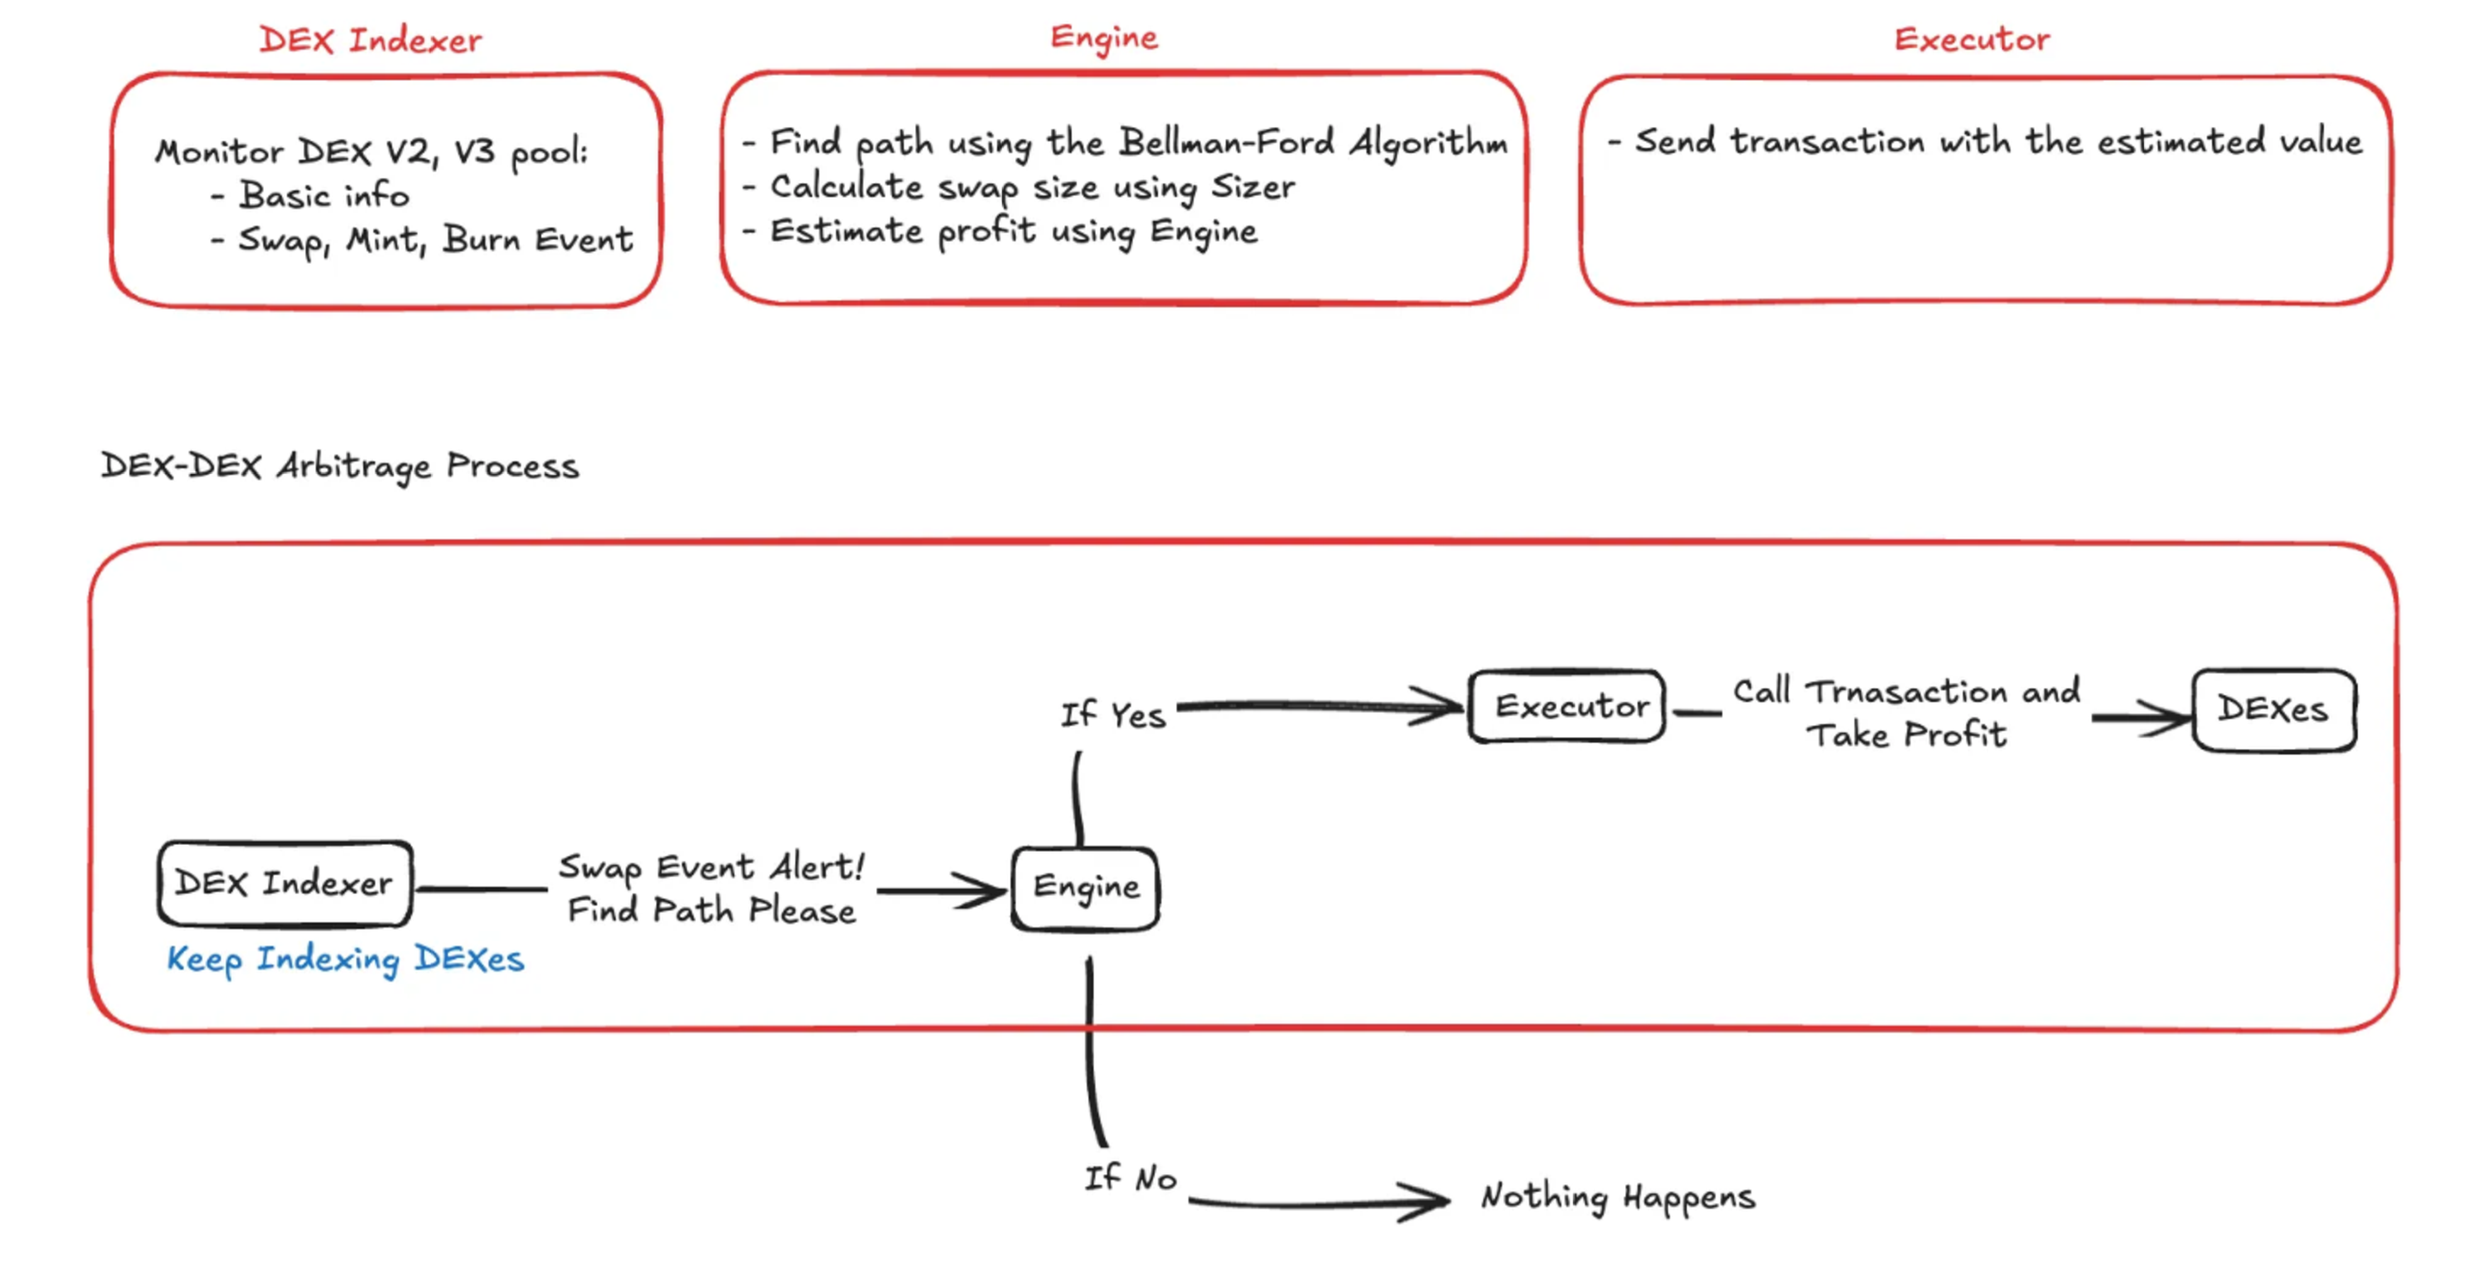
\includegraphics[width=\textwidth]{./images_goal_1/orakle_mev_architecture.png}
\end{frame}

\begin{frame}{Requirements \& Strategies}
  \begin{itemize}
    \item Low Latency $\Rightarrow$ Colocation (AWS at Tokyo)
    \item Fast \& Efficient Pathfinding $\Rightarrow$ Caching Pool Data
    \item Precise Calculation $\Rightarrow$ Reuse of battle-tested libraries and custom implementation of long-tail DEXes
    \item Top-of-Block Inclusion $\Rightarrow$ Higher Priority Fee
    \item Cost Minimization $\Rightarrow$ Custom smart contract
  \end{itemize}
\end{frame}

\begin{frame}{Results}
  \centering
  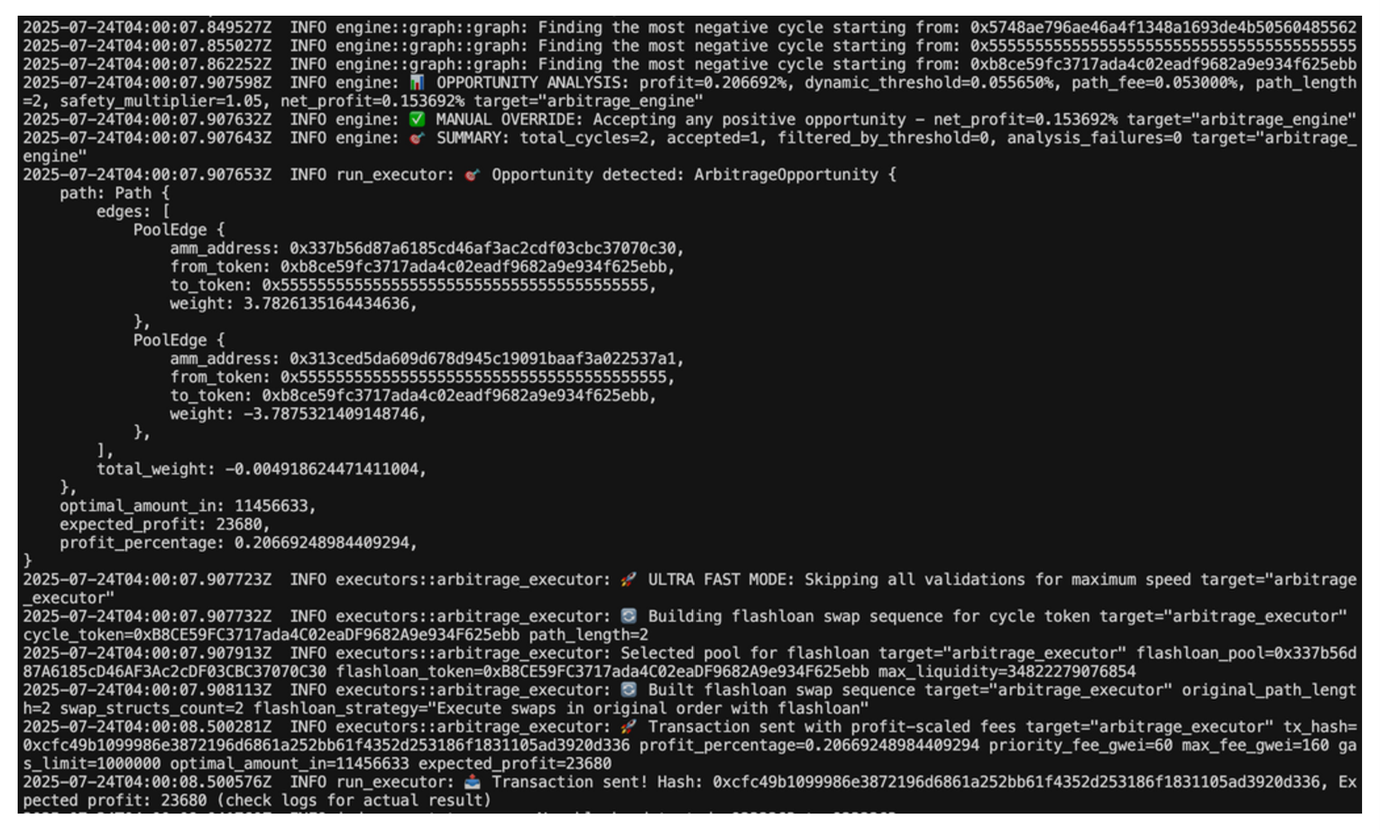
\includegraphics[width=\textwidth]{./images_goal_1/trace.png}
\end{frame}

\begin{frame}{Results}
  \centering
  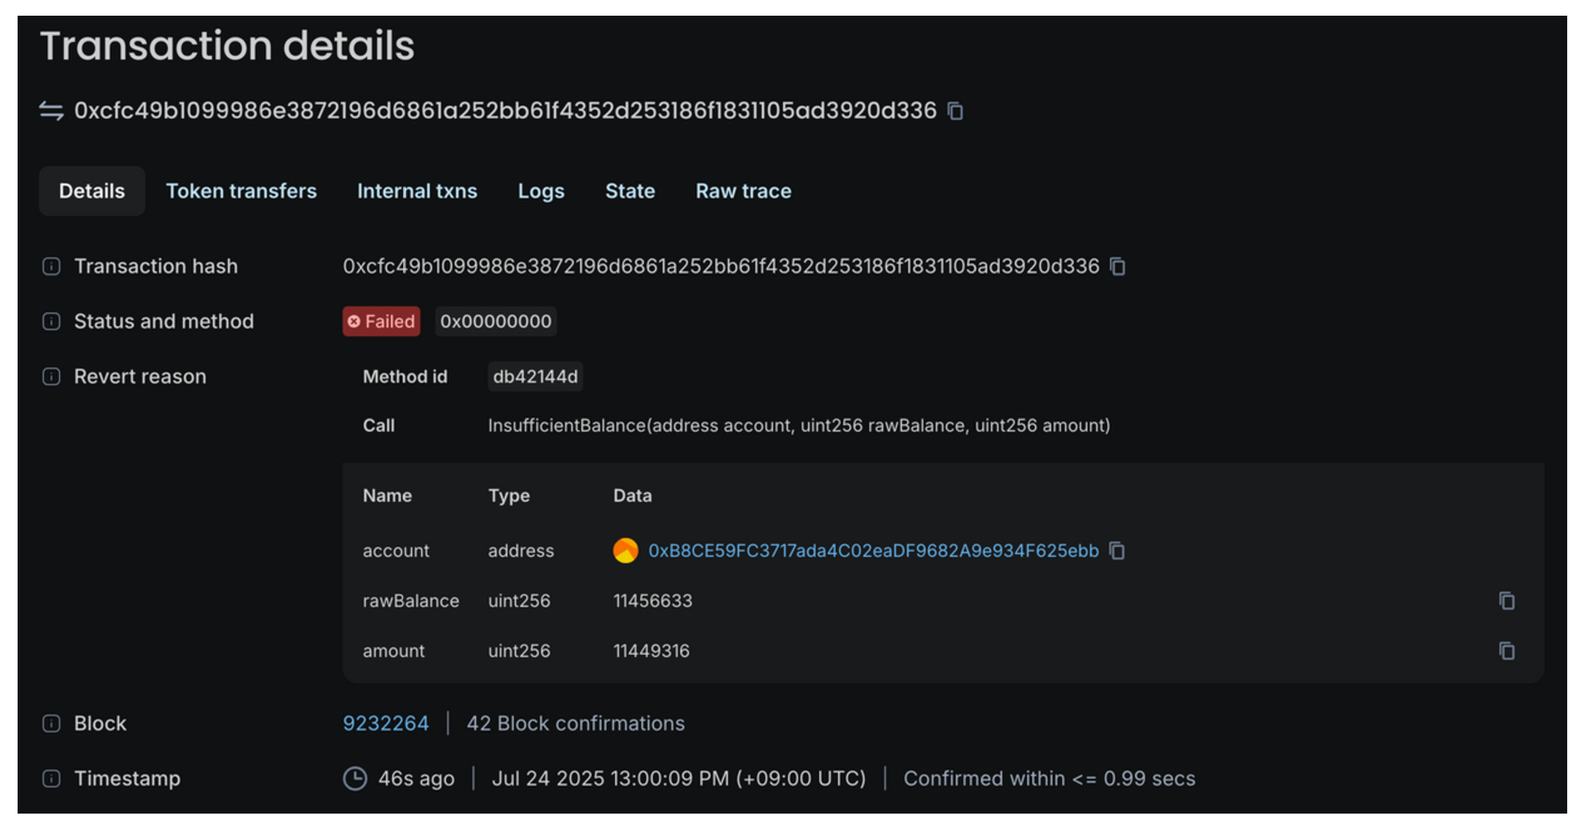
\includegraphics[width=\textwidth]{./images_goal_1/explorer.png}
\end{frame}

\section{Goal 2: Empirical Analysis}

\begin{frame}{Questions}
  \begin{itemize}
    \item Who?
    \item Why?
    \item How much?
  \end{itemize}
\end{frame}

\begin{frame}{Data}
  \begin{itemize}
    \item HYPE-USDT Pair only (Why?)
    \item Every swap in August 2025
    \item Orderbook Data: Tardis.dev
    \item Transaction Logs: eth\_getBlockReceipts from archive node provided by QuickNode
  \end{itemize}
\end{frame}

\begin{frame}{Methodology}
  \begin{itemize}
    \item Calculate mid-price as weighted mean of BBOs
    \item Calculate PnL as 1-second markout minus gas fee
    \item Judge as Searcher if:
      \begin{itemize}
        \item Cumulative PnL is positive
        \item More than 30 transactions (1 per day)
      \end{itemize}
    \item Volatility (Variance) is calculated as 1 minute realized variance
  \end{itemize}
  \centering
  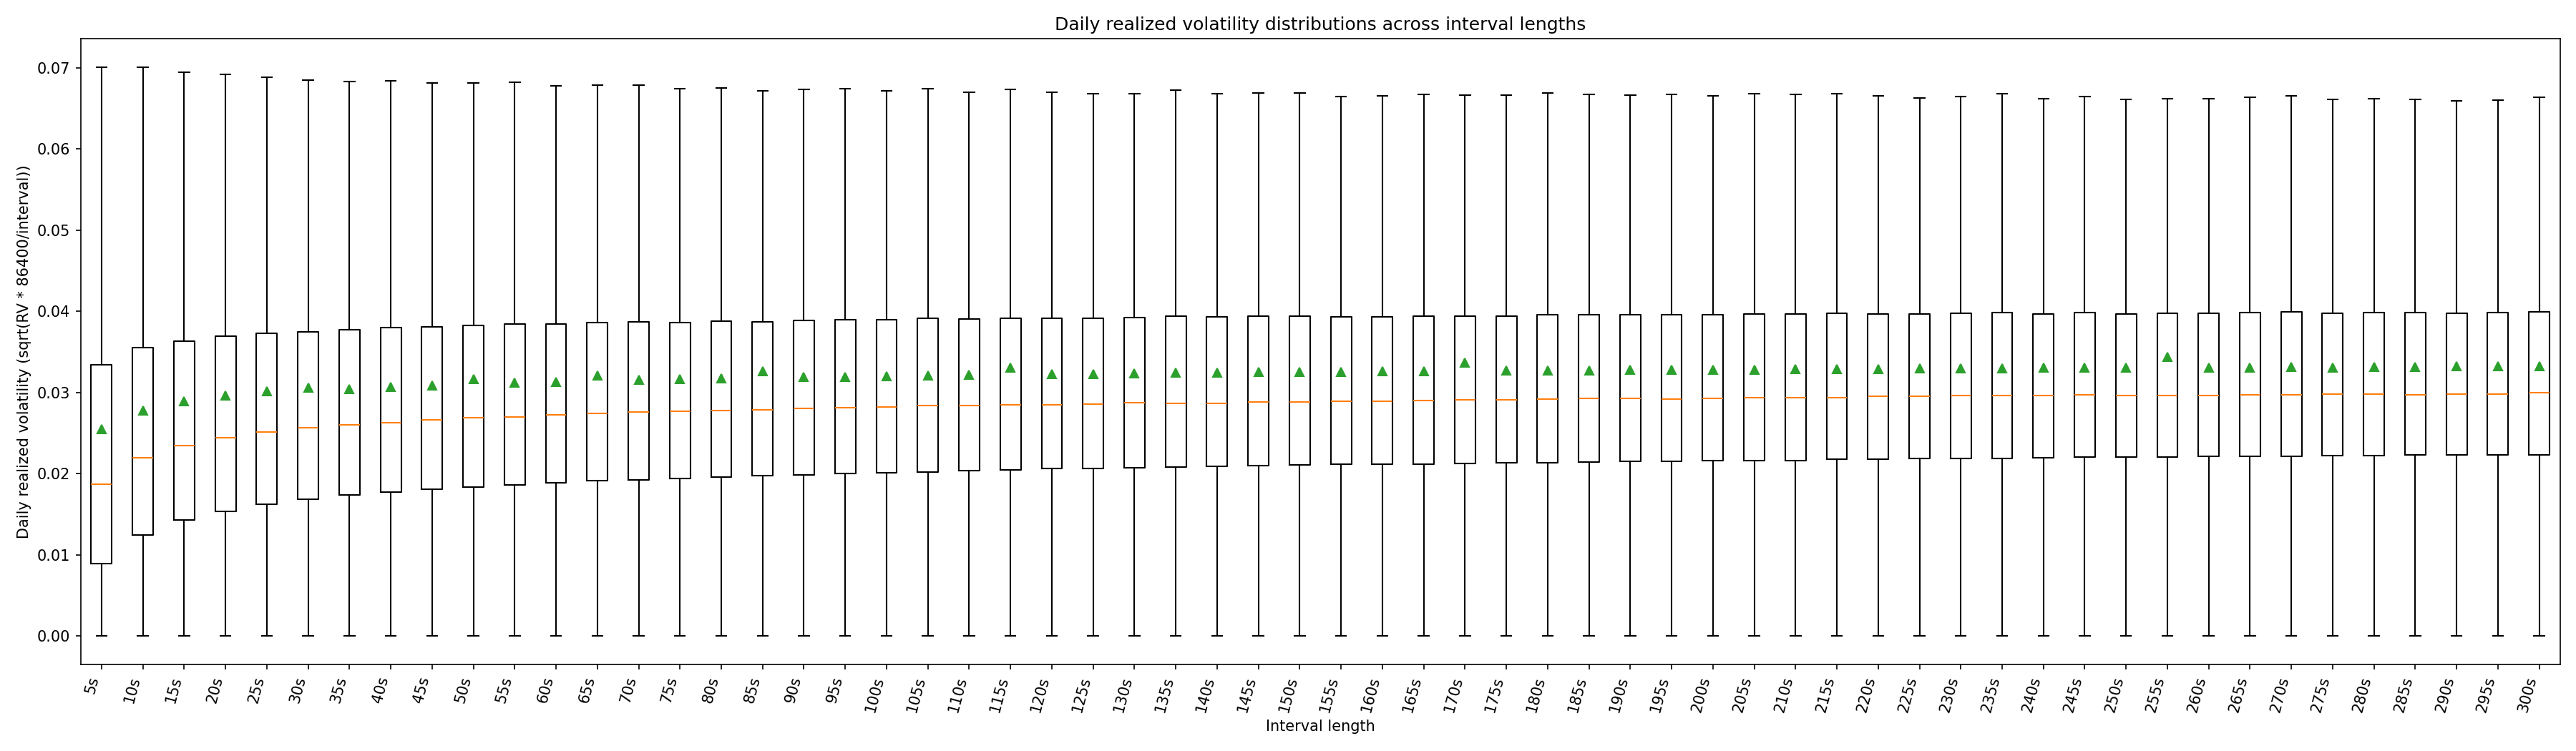
\includegraphics[width=\textwidth]{./images_goal_2/rv_boxplot_by_interval.png}
\end{frame}

\begin{frame}{Results}
  \centering
  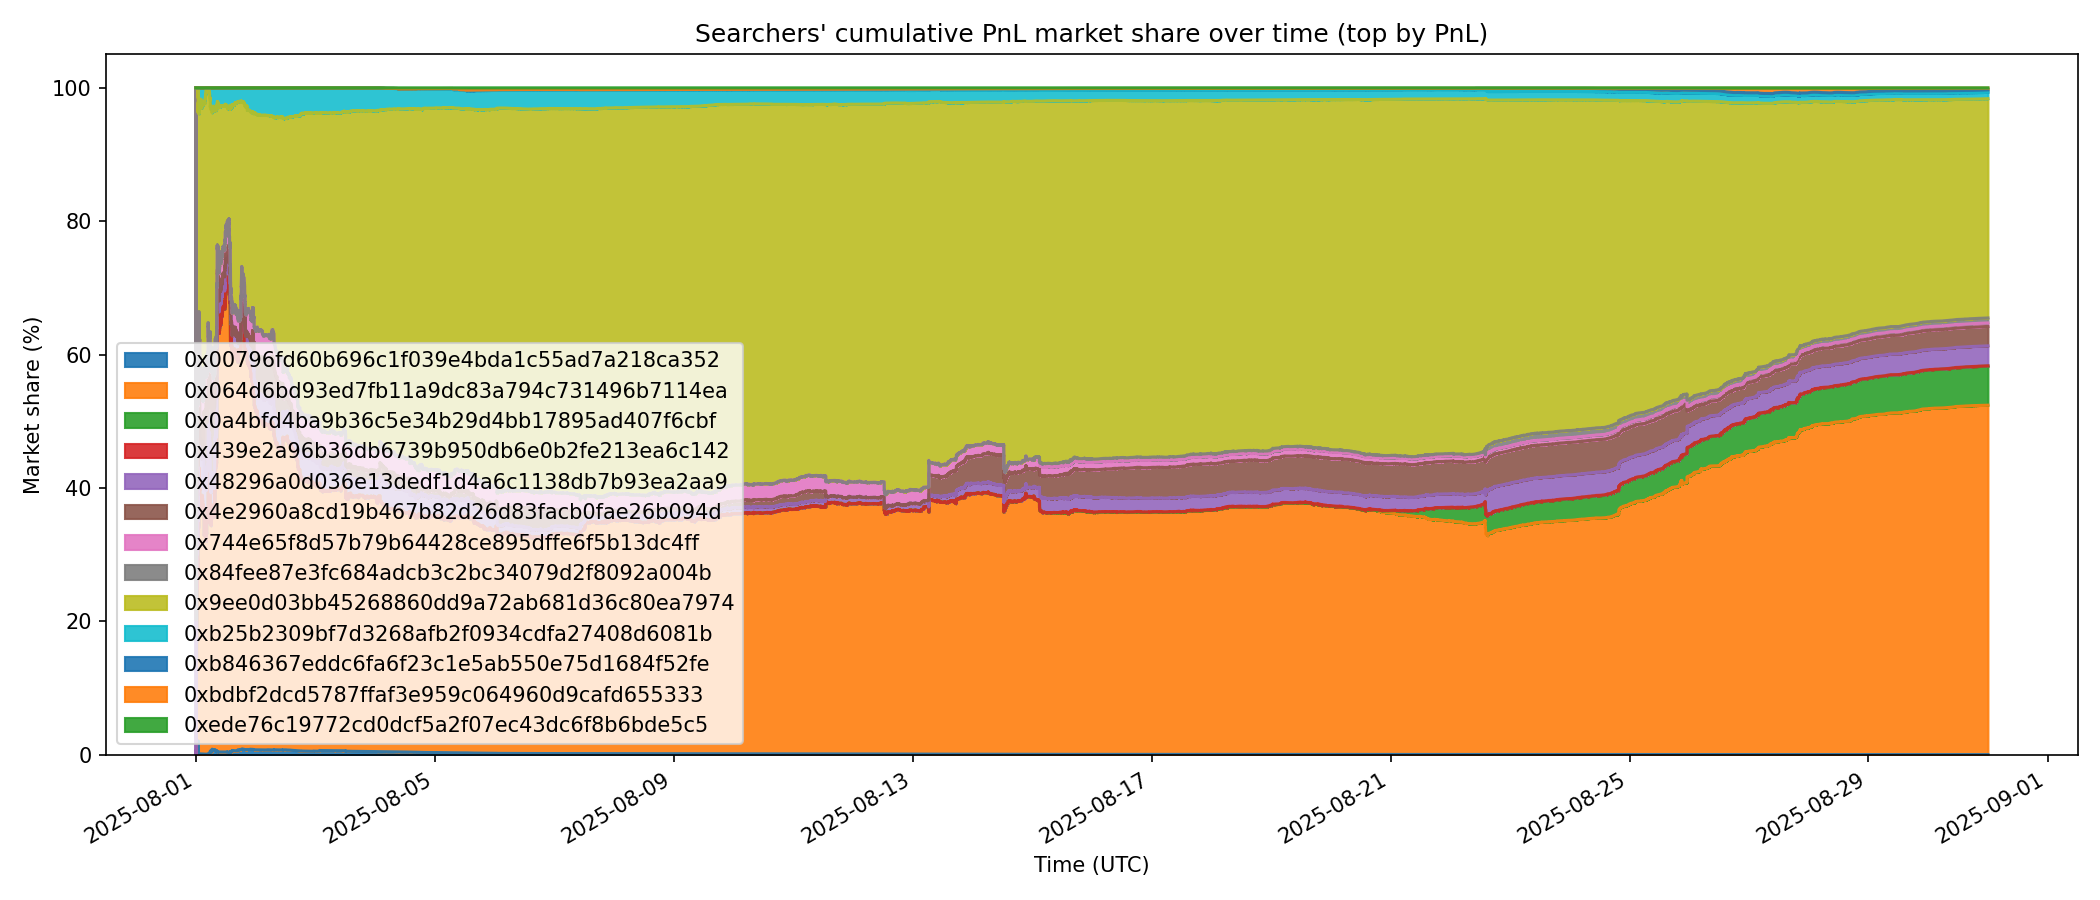
\includegraphics[width=\textwidth]{./images_goal_2/market_share_over_time.png}
\end{frame}

\begin{frame}{Results}
  \centering
  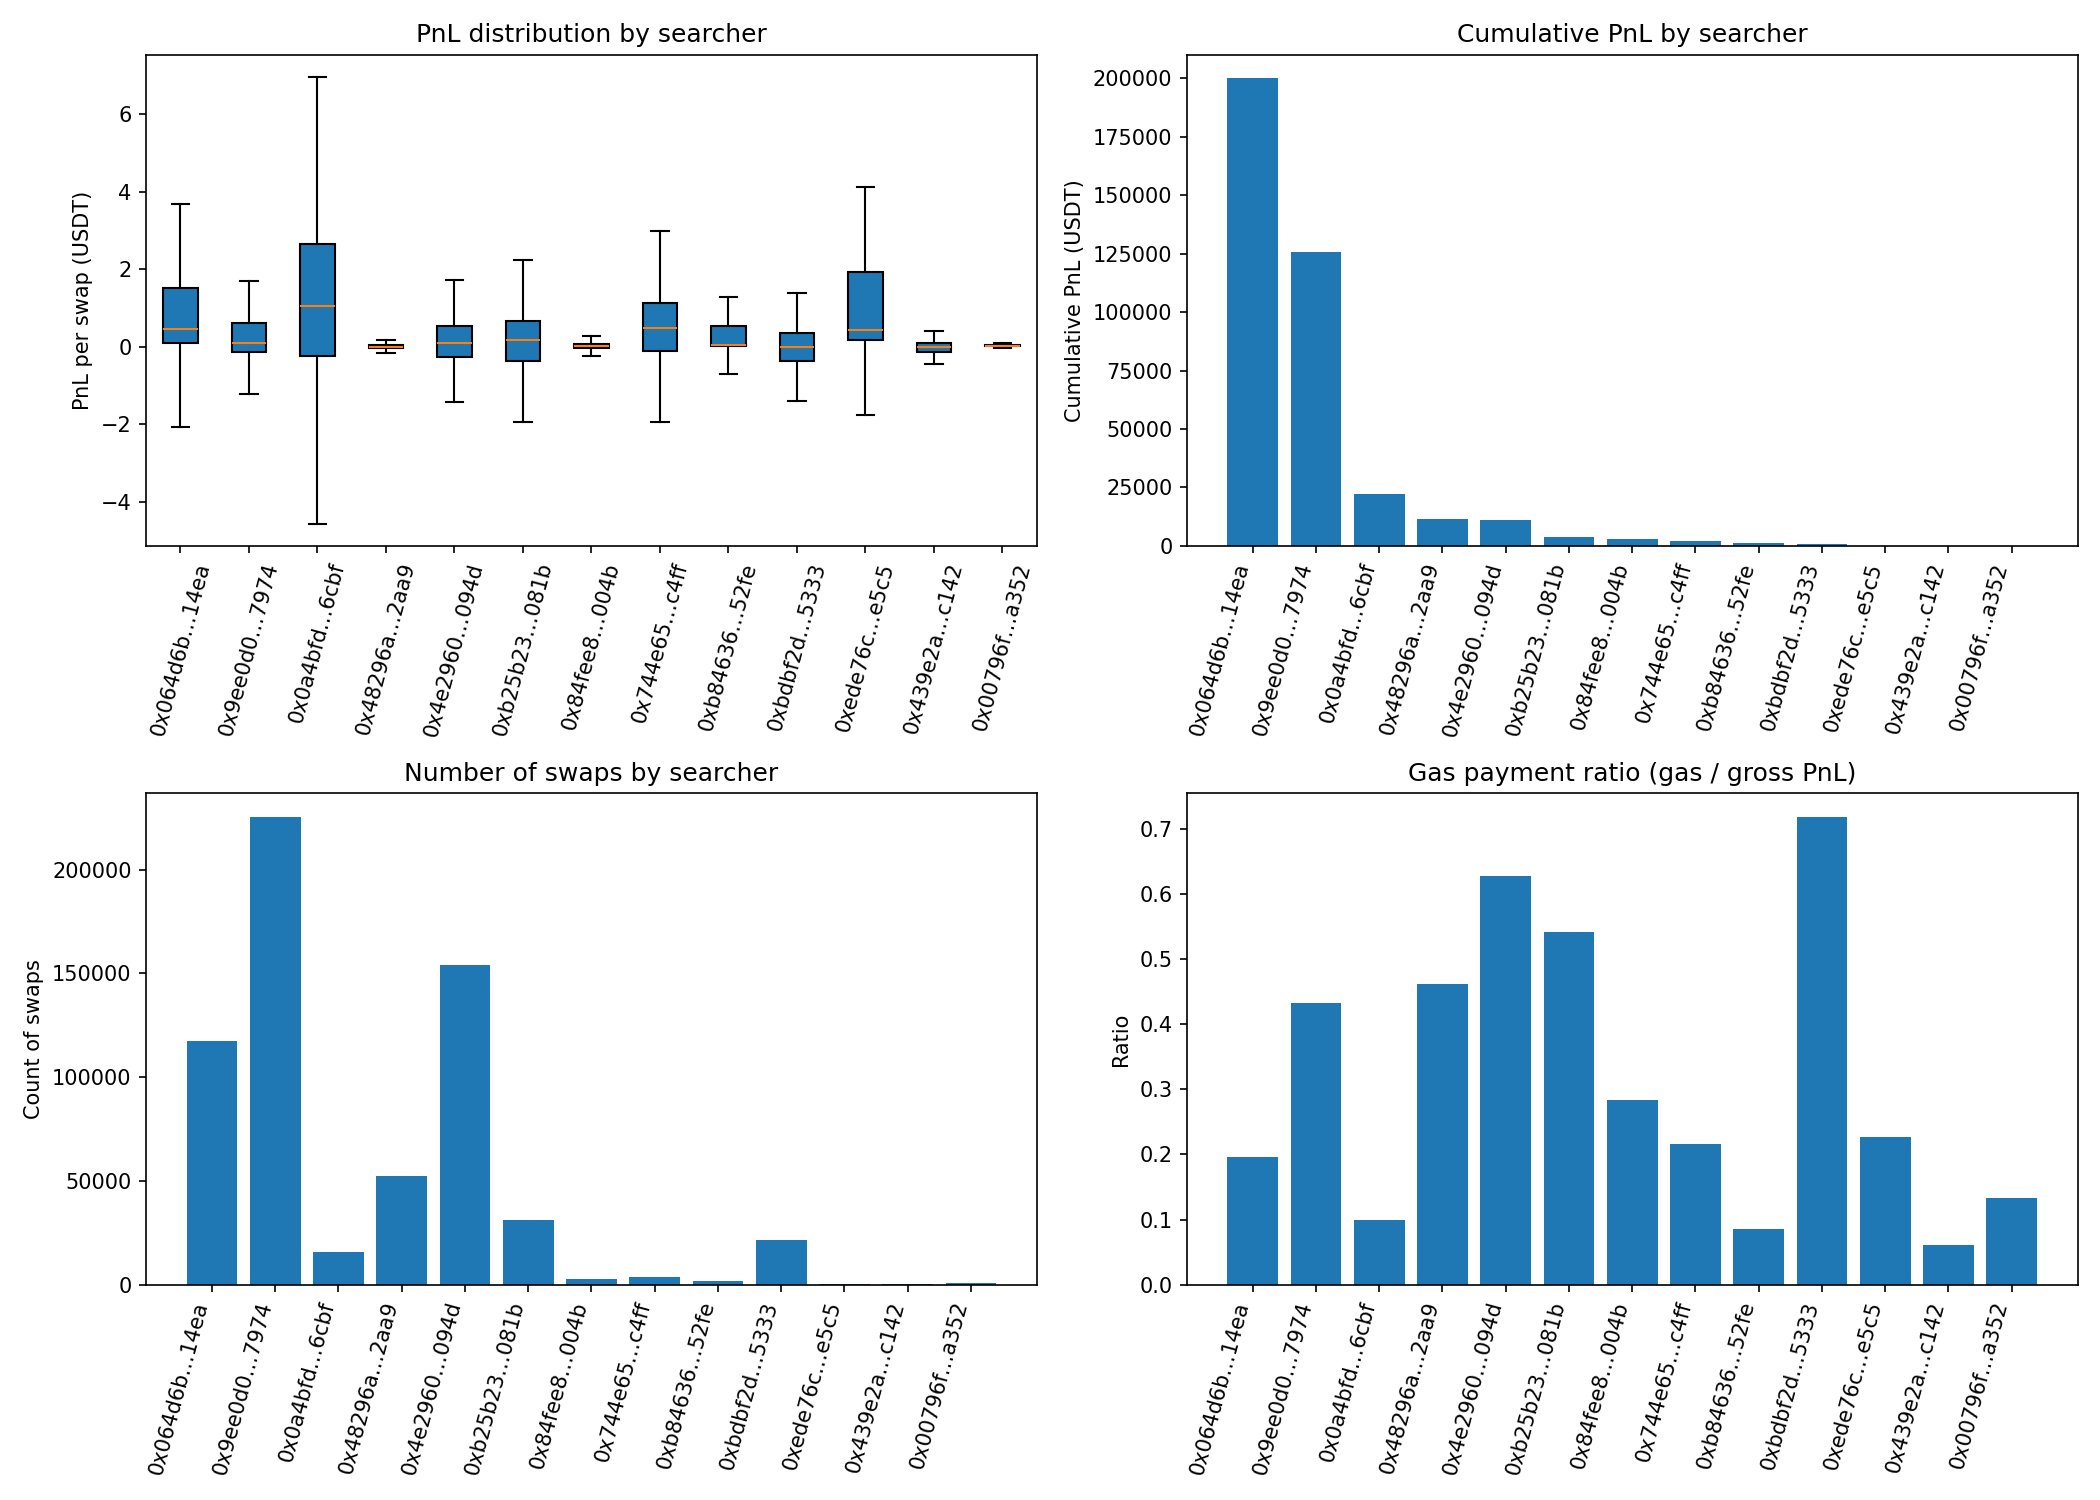
\includegraphics[height=0.8\textheight]{./images_goal_2/searcher_panels.png}
\end{frame}

\begin{frame}{Results}
  \centering
  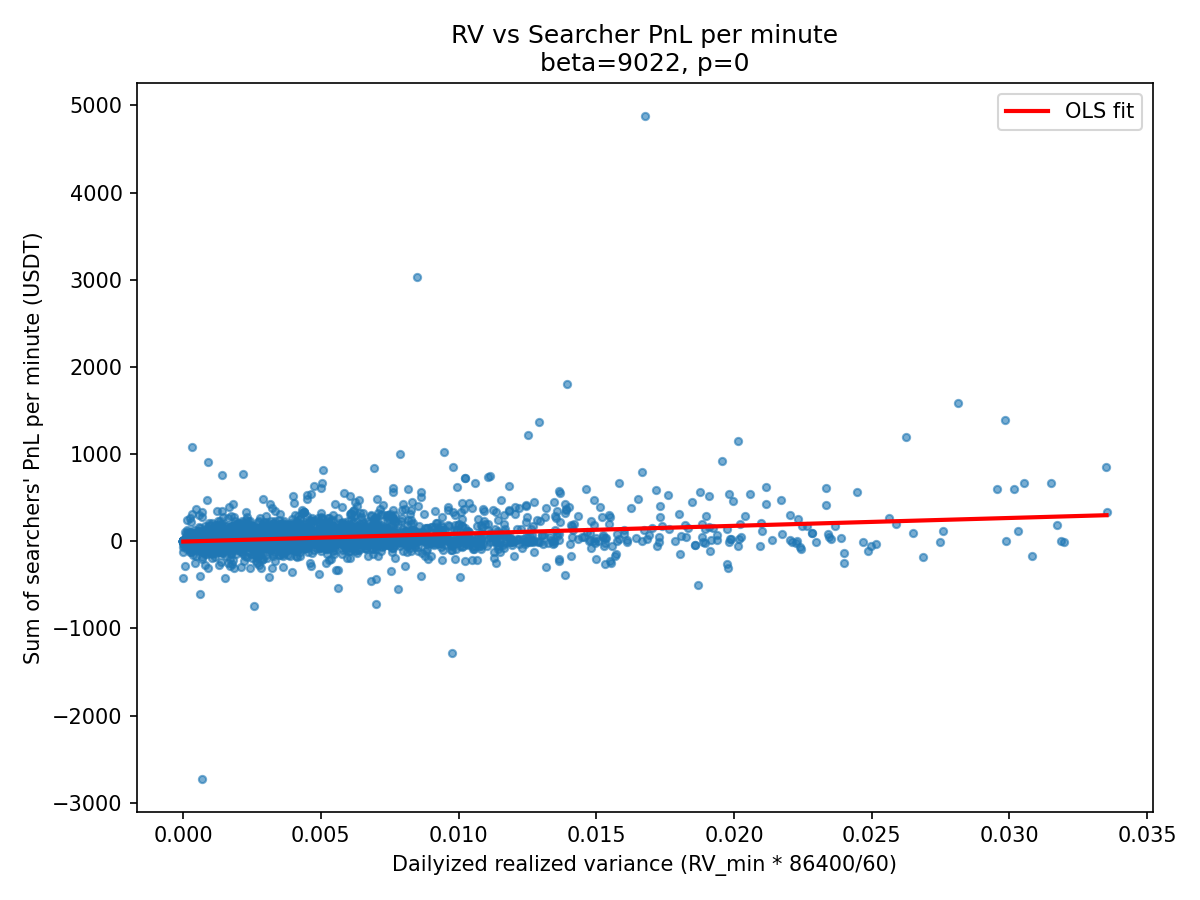
\includegraphics[width=0.8\textwidth]{./images_goal_2/rv_vs_searcher_pnl_per_minute.png}
\end{frame}

\section{Conclusion}

\begin{frame}{Conclusion}
  \begin{itemize}
    \item We tried searching for MEV on HyperEVM but failed
    \item Market was already highly competitive and dominated by top 2 players
    \item Classical result of relation between volatility and informed trading was confirmed again
  \end{itemize}
\end{frame}

\begin{frame}
  \centering
  Thank you!
\end{frame}

\end{document}